\section{Введение}
\label{sec:Chapter1} \index{Chapter1}
Аргументационная теория, или аргументация, является междисциплинарным исследованием о том, как выводы могут быть достигнуты через череду логических рассуждений. Извлечение аргументации – область науки, стоящая на стыке обработки естественного языка, информационного поиска и непосредственно аргументационной теории.

В общем виде аргумент состоит из утверждения и набора предпосылок, связанных с этим утверждением. Утверждение и предпосылки называются компонентами аргументации. Связи между ними могут выражать не только структуру аргумента, но и тип отношений внутри нее – поддержку или опровержение (атаку). Данные отношения называются полемической позицией аргументации.
\begin{figure}[H]
 \setcounter{figure}{0}
 \captionsetup{justification=raggedright,singlelinecheck=false,labelfont=bf,labelsep=period,name={Рисунок}}
 \centering{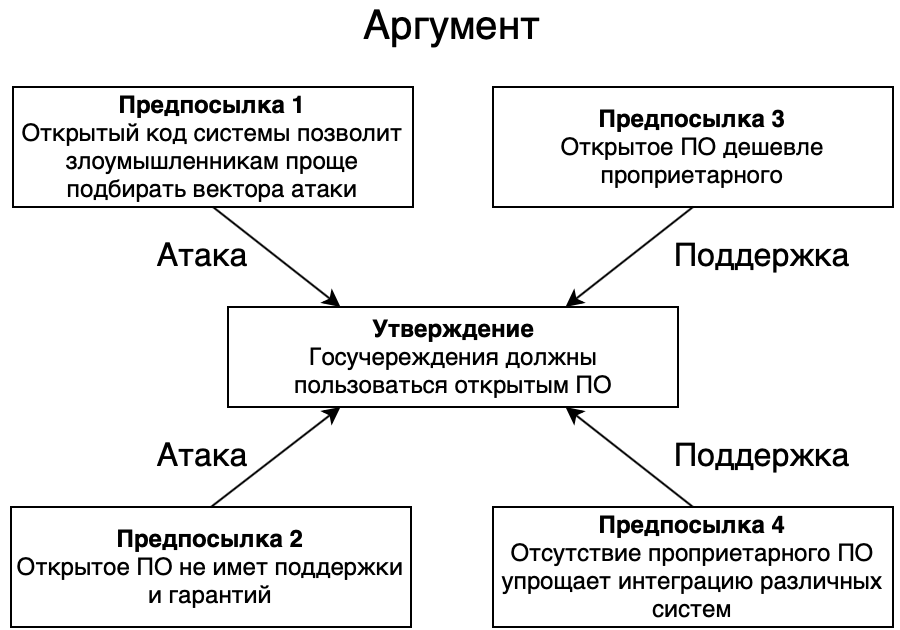
\includegraphics[scale=0.65]{argument.png}}
 \caption{Пример аргумента, относящегося к применению открытого ПО.}
\end{figure}
Аргументация присутствует почти во всех источниках информации: она встречается в бытовых спорах, дебатах, научном дискурсе. Особый вид политической аргументации – пропаганда является ключевым компонентом некоторых интернет-ресурсов.

За последнее десятилетие сильно вырос интерес к автоматическому выделению аргументации \cite{lippi2016argumentation}. Этому поспособствовал прорыв в области обработки естественного языка, заключающийся создании предобученных моделей с сильными обобщающими способностями \cite{mikolov2013efficient, devlin2018bert, radford2019language}. Несмотря на то, что данные модели содержат в себе знание общеизвестных и часто встречаемых фактов, выученных из больших коллекций \cite{petroni2019language}, они не способны применять узкоспециализированую информацию. Для решения данного недостатка используют графы знаний и другие онтологии \cite{sorokin2018modeling, chen2019multi}, однако их создание требует трудоемкий и долгий процесс ручной разметки данных экспертами. Автоматическое извлечение аргументации позволяет динамически извлекать специализированную информацию и структурировать ее.

%Cуществует несколько десятков англоязычных корпусов извлечения аргументации, решающих задачу в различных постановках, однако почти отсутствуют их русскоязычные аналоги. Проблему плохого покрытия языка можно решать созданием новых или параллельных \cite{fishcheva2019cross}  корпусов, а также методикой crosslingual transfer \cite{ponti2020xcopa, eriguchi2018zero}. Данный подход заключается в обучении мультиязычной модели на одном языке для адаптации полученных знаний на другом языке.

%В данной работе описывается исследование методов извлечения структуры и полемической позиции аргументации, а также способы адаптации данных методов для применения на русскоязычных корпусах с помощью подхода crosslingual transfer.

\subsection{Актуальность задачи}
Извлечение аргументации можно применить во многих прикладных сценариях:
\begin{itemize}
    \item Аргументация может быть задействована в экспертных системах для получения доводов "за"  и "против" относительно какого-либо утверждения.
    \item Аргументы можно использовать в голосовых помошниках и других системах, использующих базы знаний.
    \item Выделение аргументации применительно к научным текстам позволит лучше высторить структуру взаимосвязи между цитируемыми работами.
    \item Аргументация также может использоваться для оценки убедительности и логичности текстов.
\end{itemize}

Научная ценность данной работы заключается в исследовании и систематизации текущих подходов к задаче извлечения аргументации и адаптации англоязычной модели для работы с русскоязычными текстами. В работе также проводится интерпретация работы модели: исследуется зависимость полученных результатов в зависимости от структурных особенностей компонент аргументации, таких как наличие отрицаний, сильно окрашенных слов или антонимии.

\subsection{Постановка задачи}
Целью данной работы является исследование методов извлечения аргументации в текстах и создание аналогичных систем для русского языка. Для решения поставленой цели необходимо решить следующий подзадачи:

\begin{enumerate}
	\item Произвести обзор существующих решений и корпусов.
    \item Воспроизвести избранные работы или получить новые базовые решения.
    \item Предложить методику для получения русскоязычной модели извлечения аргументации.
    \item Провести анализ полученной модели с целью интерпретации полученных результатов.
\end{enumerate}


\subsection{Обзор существующих исследований и  решений}
Задачу извлечения аргументации можно разделить на 2 подзадачи: выделение компонент аргументации и определения отношений между ними. Подход к решению этих задач достаточно сильно различается в разных работах, что приводит к невозможности объединения всех корпусов в один.

Например, в работах \cite{aharoni2014benchmark, rinott2015show, levy2018towards} предлагается следующая постановка задачи: по заданной теме необходимо найти контекстно-зависиое утверждение, к утверждению необходимо найти контекстно-зависимые предпосылки. Данные термины имеют следующие определения:
\begin{itemize}
    \item Тема - короткая противоречивая фраза, определяющая центральный объект обсуждения.
    \item Контекстно-зависимое утверждение - краткая фраза, напрямую подтверждающая или опровергающая тему.
    \item Контекстно-зависимая предпосылка - участок текста, напрямую поддерживающий или опровергающий контекстно-зависимое утверждение в рамках данной темы.
\end{itemize}

В последующей работе от тех же авторов \cite{ein2020corpus} происходит упрощение модели аргументации за счет объединения темы и контекстно-зависимого утверждения. Задача заключается в нахождении предпосылок по заданным утверждениям.

В работе \cite{lippi2015context} предлагается извлечение контекстно-независимых утверждений, которые впоследствии нужно соотносить с различными темами. В работе \cite{bar2017stance} предлагается классифицировать отношения поддержки и опровержения между утверждениями и темами. Судебные юридические тексты из \cite{palau2009argumentation} размечены по предложениям с точки зрения отношения к предложению, отмеченному как вывод.

Помимо вышеописанных корпусов существуют размеченные речи дебатов, где размечены враждующие утверждения. Существует несколько корпусов с различными видами аргументации, размеченными в рамках научных статей (DrInventor, ScitDB). Internet Argument Corpus v2 содержит примеры интернет-дебатов, где сообщеняи размечены с точки зрения полемической позиции, наличия сарказма и эмоционального окраса.

Существуют также корпуса для определения \textit{качества} аргументов \cite{toledo2019automatic, gretz2020large}. Данные корпуса содержат утверждения и относящиеся к ним пары предпосылок с указанием того, какая из предпосылок лучше.

Дополнительно стоит отметить и примеры политической аргументации, содержащиеся в корпусе трека SemEval 2020 Task 11 Propaganda detection in news articles. В данном соревновании предлагается выделить участки новостных статей, содержащих аргументацию, а также классифицировать их в такие приемы, как ложная аналогия, подмена тезиса, эксплуатация двусмысленных выражений, сведение аргументации к универсально осуждаемой теме и другим приемам убеждения оппонента.

Отдельной постановкой задачи отличается и корпус Webis Debate 16\cite{webis16}. Данный корпус является коллекцией фраз размеченных бинарным образом как нейтральные и содержащие аргумент.

Было создано несколько полноценных систем для извлечения аргументации, работающих с различными постановками задачи:
\begin{itemize}
    \item MARGOT - данная система придерживается определений контекстно-зависимых утверждений и предпосылок. По заданной теме к тексту последовательно применяется несколько моделей - модель определения предложений, содержащих компоненты аргументации, и модель выделения компоненты внутри предложения.
    \item Targer - система аналогичная MARGOT по постановке задачи. Используется единственная модель для классификации слов в тексте для выделения компонент аргументации.
    \item ArgumentText - данная модель ближе ко второй модели аргументации; по заданной теме она ищет предложения и классифицирует в классы поддержки и атаки.
\end{itemize}

По причине большого объема и довольно разнородных подходов на данный момент не были исследованы следующие корпуса:
\begin{enumerate}
    \item Корпуса Webis.DE - Arg-Microtexts, args.me corpus, ArguAna Counterargs, ArguAna TripAdvisor.
    \item Корпуса IBM - саммаризация аргументов в ключевые позиции; корпуса классификации по абстрактности и противоречивости; корпуса по кластеризации и сентименту; корпуса по расширению темы аргумента; корпуса по определению экспертной позиции; корпуса размеченных речей, полученных из дебатов.
    \item Корпуса UKP - размеченные с точки зрения аргументации эссе, отзывы на продукты, статьи, диалоги.
    \item Корпуса с соревнований CLEF и FEVER.
\end{enumerate}


Несмотря на довольно большой список работ, посвященных извлечению аргументации, использование больших предобученных моделей по типу BERT \cite{devlin2018bert} остается слабоисследованным, как и анализ возможности переносимости подобных систем на русский язык.

\subsection{Ход работы}

Планируется обработать англоязычные корпуса для получения объединенного англоязычного корпуса аргументации. На различных комбинациях задач планируется исследовать применимость различных подходов к извлечению аргументации.

Для интерпретации полученных результатов разрабатывается веб-приложение, которое позволит в интерактивном режиме анализировать поведение модели.

Для решения задачи переноса знания на русский язык изучаются подходы описанные в работах \cite{conneau2018xnli, nooralahzadeh2020zero, schuster-etal-2019-cross-lingual}. Данные подходы основаны на применении предобученных мультиязычных моделей, их дообучении в низкоресурсных сценариях, а также дистилляции знаний. Для оценки эффективности методов планируется перевод некоторых корпусов на русский язык.

Таким образом рассматривается задача создания русскоязычной модели извлечения аргументации, для решения которой используются методы, предложенные в работах \cite{nooralahzadeh2020zero, schuster-etal-2019-cross-lingual}, так как они успешно зарекомендовали себя в задачах семантического вывода, которые близки к задаче выделения структуры и полемической позиции аргументации.
